\documentclass[12pt,relax]{PetraObjectModel}
% ---------------------------------------------------------------------------- %
%
% Set the title, author, and date
%
\title{The Petra Object Model for Parallel Linear Algebra Computations}
\SANDsubtitle{}

\author{Michael A.~Heroux, Robert J. Hoekstra and Alan Williams \\
	   Sandia National Laboratories\\
	   P.O. Box 5800\\
	   Albuquerque, NM 87185-1110
	 }

% There is a "Printed" date on the title page of a SAND report, so
% the generic \date should generally be empty.
\date{}


\SANDnum{SAND2003-xxxx}
\SANDprintDate{February 2003}
\SANDauthor{Michael A.~Heroux \\
Computational Mathematics and Algorithms Department \\
 \\
Robert Hoekstra \\
Computational Sciences Department \\
 \\
Alan Williams \\
High Performance Computing and Networking Department \\
 \\
Sandia National Laboratories \\
P.O. Box 5800 \\
Albuquerque, NM 87185-1110}



\SANDreleaseType{Unlimited Release}


\begin{document}
\maketitle

\begin{abstract}
This paper describes the design and implementation of a parallel, 
distributed memory, object oriented model for basic
matrix and vector services required for the solution of linear, 
non-linear and evolutionary problems which arise in scientific 
and engineering applications.  We first provide an overview of 
the basic object model using the Unified Modeling Language (UML), 
and then discuss in detail several implementations.
\end{abstract}


\clearpage
\section*{Acknowledgement}
The author would like to acknowledge the support of the ASCI and LDRD programs
that funded development of Trilinos.

\newpage
\
\vspace{3.5in}
\begin{center}Intentionally Left Blank\end{center}
\clearpage
\tableofcontents
\listoffigures

\clearpage
\addcontentsline{toc}{section}{Nomenclature}
\section*{Nomenclature}
\begin{itemize}
\item[Processor] A computing element that can execute compiled 
code and directly access some physical memory resource.  Typically 
a processor is one of the commonly available commodity microprocessors.

\item[Process] An executable file submitted to the operating system.  
A process must be assigned to a processor in order to execute.  At 
any given time, it may be running on a processor or sitting idle in 
memory.

\item[Node] A computing element that has a single, usually 
hardware-supported, address space.  In other words, a processor 
on a node can directly address any memory location on the node.  
A node has one or more processors, all of which have access to the 
same shared memory.  Typically a node is a single integrated hardware 
unit that, in other customer situations, would be sold as a
stand-alone 
system.

\item[Memory Image]  Some portion of memory existing on a single node.
This memory is associated with one or more processes.


\item[Parallel Machine] For our purposes a parallel machine is a
collection of $l$ nodes, where the $i^{th}$ node has $k_i$ processors that have 
shared memory.  The total number of processors is 
\begin{equation}
p = \sum_{i=0}^{l-1} k_i
\end{equation}

\end{itemize}

\newpage

\section{Introduction}


Many numerical algorithms for the solution of problems in 
scientific and engineering applications use vectors and 
matrices as basic elements.   Generally, the exact details 
of how these mathematical objects are stored, or how computations 
are performed using them, is not of primary importance for the 
algorithm designer.  Because of this, using abstract object models 
that describe the attributes and methods associated with each 
object class, and defining the relationship between classes, is an 
effective way to separate algorithm design and implementation from 
vector and matrix design.

The practical importance of this separation comes from the fact 
that there are many different data structures used to store 
vectors and matrices and correspondingly many different ways 
to implement basic matrix and vector operations.  The variety 
of vector matrix data structures and implementations is, to 
some extent, a result of arbitrary choices made by application 
designers.  However, often there are sound reasons for choosing 
particular data structures, either because of the intended 
computer architecture or because of the specifics of the 
application.  Abstraction of the vector and matrix objects 
leverages the investment in sophisticated algorithm implementations 
across many different vector and matrix implementations and 
provides a convenient generic programming framework for new 
algorithm development.

In this paper we present a detailed object model for vectors 
and matrices that are intended for use in a parallel, distributed 
memory computing environment.  We present a brief overview of 
the classes in the next section followed by a detailed UML object 
model in the next section.  In subsequent sections we will present 
a collection of pure virtual classes, two C++ implementations of 
this model and a Java implementation.


\section{Overview of Primary Petra Classes}

In this section we present in logical order the basic object classes 
needed for parallel vectors and matrices.  Each of the object
classes represents a family of classes with one base class and 
specialization of the base class.

\paragraph{Comm Class:  Parallel Machine Description}

We begin with the Comm class that describes parallel machines.  
This class is an attribute in most other classes since it provides 
essential information and services needed for operations across the 
parallel machine.  The Comm class provides information about the number 
of  logical nodes on the parallel machine and node identification.  It 
also provides basic services such as global synchronization and collective 
communications.

\paragraph{Map Class: Object Distribution Specification}

The second class we present is the Map class.  This class is a 
specification of the distribution of a collection of global identifiers 
(GIDs).  GIDs are integer values and need not be uniquely owned by a 
processor or cover a contiguous range of integer values.  An object is 
distributed across the parallel machine by associating subsets of the 
object data with the GIDs.  Each node of the parallel machine will be 
assigned zero or more GIDs.  Example 1 illustrates this concept for the 
simple case of a distributed vector.   Each map object requires a Comm 
object to be passed in at construction.

\paragraph{Vector Class:  Vector Object}

This class allows construction and manipulation of vectors, and supports 
operations involving vectors.  Basic vector 
operations include norms, dot products, vector updates, etc.  The interface 
to the vector constructors and vector methods is independent of the specifics 
of the parallel machine and the vector distribution since this information is 
encapsulated in the map object passed in during construction.

\paragraph{Multivector Class:  Generalization of a Dense Matrix}

This class allows the construction and manipulation of a collection of 
vectors that have the same size and distribution, i.e., the same map.  
A multivector is a generalization of a dense matrix.  There are methods 
in the class that provide results for each vector in the multivector and 
methods that view the multivector as a matrix.  In a practical implementation, 
one should note that the vector class can usually be implemented as a 
specialization of the multivector class (a multivector with one vector).

\paragraph{Row-biased Graph Class:  Connectivity Graph Object}

A graph object specifies a set of vertices and the connecting edge pairs.
The graph is then constructed across a parallel machine by associating each
row of the graph with a GID and assigning the entire row of the graph to the
node(s) that owns the GID. In the Petra object model, graph objects are held
as attributes by matrix classes, and are used to define and describe the
structure of the matrix (location of nonzero entries).

\paragraph{Operator Class: Linear Operator Object}

The Operator interface is the highest-level abstraction for matrix objects,
representing only mathematical operations performed with matrices and
specifically avoiding issues relating to storage formats and implementation
details. The Operator interface is inherited and implemented by all of our
'concrete' matrix classes.  Algorithms which are written to use these
abstract Operators rather than specific matrix class types may make use of
any matrix type that implements the Operator interface.

\paragraph{Row-biased Matrix Class: Sparse Matrix Object}

A row-biased matrix is very similar to a row-biased graph.  Additionally it 
contains matrix values and has methods to compute matrix-vector and
matrix-multivector multiplications.  It also has methods to provide certain
matrix norms and scalings.  It can also be queried row-wise for matrix entries.
As will be discussed in a later section, Petra implementations include both
point-entry and block-entry matrix classes.

Figure~\ref{matvecmap} shows inheritance (solid lines) and collaborations
(dotted lines) among the Matrix, Vector and Map classes.
\begin{figure}[ht]
\begin{center}
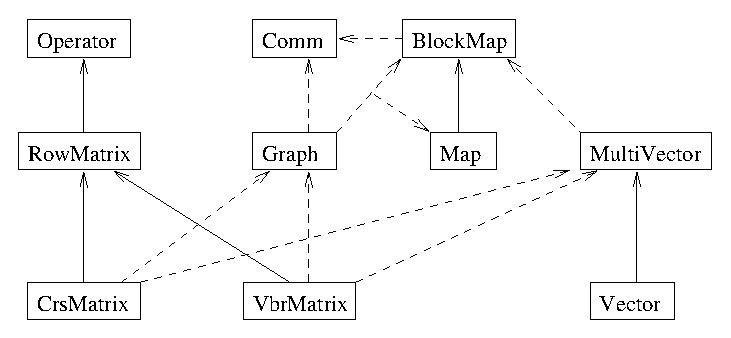
\epsfig{file=mvmcollab.eps, scale=1.0}
\caption{Matrix, Vector and Map inheritance and collaborations.}
\label{matvecmap}
\end{center}
\end{figure}

\paragraph{Import and Export Classes:  Parallel Data Redistribution}

Given a vector, multivector, graph or matrix distributed across nodes via a map (call 
it a source map), it is possible to redistribute any of these objects by creating a 
new map (a target map) and then creating an import or an export object to redistribute 
the object to the layout specified by the target map.

An import object is used in the situation where a target map is constructed using GIDs 
that the calling node want to obtain from the source map layout.  An export object is 
used when the target map is constructed so that each GID in the source map is uniquely 
owned by one node in the target map, effectively asserting that each calling processor 
wants to export anything that is in its source map but not in its target map.  Import 
and export objects form the basis for all data communication on the parallel machine.

\paragraph{Serial Dense Matrix and Vector Classes:  Serial Dense Linear Algebra Objects}

Because there are many good implementations of serial dense linear algebra operations, 
e.g. optimized BLAS on many computers, we provide an abstract class hierarchy to define 
dense matrix and vector objects.  The default implementation of these classes uses the 
standard Fortran BLAS and LAPACK interfaces~\cite{BLAS1,BLAS2,BLAS3,LAPACK}, 
but other similar libraries could be 
used, including shared memory parallel implementations of the same libraries.

\paragraph{Linear Problem Class:  Composite Class for Defining a Linear Problem}

One of the most common uses for matrix and vector classes is solving a linear system of 
equations, $AX = B$, where $A$ is a known (sparse) matrix, $B$ is a known set of one or 
more right hand side vectors and $X$ is the corresponding set of initial solution 
guesses (if any).  To facilitate this process, we define a composite linear problem 
class that contains an abstract row-biased matrix object (the base class of our 
row-biased class and block row-biased matrix classes), a multivector (which could be a 
vector since multivector is the base class for vectors) containing the right hand side 
and another multivector containing the initial guess.

\section{Parallel Machine Interfaces and Implementations}

\subsection{The Comm and Related Interface}

\subsubsection{The Comm Interface}
\subsubsection{The Directory Interface}
\subsubsection{The Distributor Interface}

\subsection{Parallel Machine Implementations}
\subsubsection{Serial Implementation}
\subsubsection{MPI Implementation}
\subsubsection{LBComm Implementation}
\subsubsection{MPI-SMP Implementation}
\subsubsection{Future Implementations}


\section{Index Spaces}
We define a vector to be a list of elements, with each element being a
dense block of one or more real-valued numbers. The set of indices used to
address the elements in a vector is referred to as an index space. Matrices
in general have two index spaces, one for the domain and another for the
range. Matrices and vectors may be used together in operations (such as
matrix-vector products) if they share compatible index spaces. Matrices
and vectors which are distributed across multiple processors must have
distributed index spaces.

\subsection{Defining Index Spaces}
In the Petra object model, index spaces are defined and described using the
Map class. The Map class describes not only global properties such as total
number of elements, but also distribution and partitioning properties such as
number of local elements (local to a particular processor), etc.
 
There are a number of ways to define a distributed index space using Petra
Maps. Depending on how the indices are assigned to processors, the distribution
may be described as uniform or non-uniform, and linear or general.

\subsubsection{Uniform vs Non-Uniform Index Space Distributions}
A uniformly distributed index space has an equal number of indices assigned
to each processor. (In cases where the number of indices is not an integer
multiple of the number of processors, then some processors may have 1 fewer
indices than other processors.) A non-uniformly distributed index space has
have arbitrarily varying numbers of indices assigned to each processor at
the discretion of the user.

\subsubsection{Linear vs General Index Space Distributions}
An index space has a linear distribution if indices are distributed across
processors in contiguous ordered groups. In this case, the first global index
on processor with rank $p$ is one greater than the last global index on
processor $p-1$. An index space with
a general distribution has indices in arbitrary order, as defined by the user.

\subsection{Block Index Spaces}
In cases where the corresponding vector or matrix has block-elements (elements
which consist of more than one point-entry) we describe the index space as a
block index space, and the appropriate Petra class is called a BlockMap. The
BlockMap class is a generalization of the Map class (a Map is equivalent to a
BlockMap with all element-sizes equal to 1). A BlockMap allows the user to
specify the element-sizes at construction, and provides query methods for
obtaining element-sizes corresponding to given elements referred to using
global identifiers (GIDs).

\section{Vectors and MultiVectors}
In the Petra object model, the Vector class is defined to have dense,
real-valued entries or elements. Each Vector object has a Map or BlockMap as
an attribute.  Vector objects are distributed across the 
parallel machine at construction by passing the map into the constructor.  
The number of GIDs in the map determines the global length of the vector 
(although a more general map class will allow multiple vector entries to 
be associated with a single GID), and the list of GIDs on each processor 
determines the segment of the vector stored on the processor.

\subsection{MultiVectors as Distributed Dense Matrices}
A Petra MultiVector is a collection of Vectors. A MultiVector is a
generalization of the Vector class and supports the
same operations as a Vector, such as norms, dot-products etc. A MultiVector
allocates memory for its collection of vectors using a contiguous array which
is identical to a two-dimensional Fortran array. This provides significant
advantages in providing access to selected dense BLAS and LAPACK operations.

\section{Compressed Index Sparse Graphs}
A Petra Graph is used to define the nonzero structure of Petra matrices. The
matrix classes each hold a Graph object as an attribute.
In general, our graphs are directed acyclic graphs (DAGs), so that one must
specify the direction of the connectivity between two vertices.  A graph is
often used to describe the connectivity of a sparse matrix, independent of
the values of the matrix, such that the connectivity graph of the matrix has
a directed edge from vertex $i$ to vertex $j$ if matrix $a_{ij}$ is nonzero.

Once a graph is constructed and filled, it can be used to determine
communication patterns and perform any setup procedures that would improve
the performance of basic sparse matrix operations for matrices that become
associated with the graph.  As part of this setup, the graph will construct
an import map and an import object (described below), that allows for
efficient communication during a sparse matrix vector multiplication.

A graph requires a map to be passed in at construction time.
In addition to passing in a map, one may provide
information about how many nonzero entries will be inserted into each row 
of the graph on each processor.  This information can be helpful for
performance, but is not required, nor is it a fatal error if the estimate
is incorrect.  One should note that a row may be owned by more than one node.

\subsection{Row vs Column Orientation}
A row-oriented graph can be thought of as a collection of rows, where each row
contains a list of column-indices. Each row is wholly owned by the local
processor. A row-oriented graph is distributed across processors by assigning
sets of complete rows to the various processors. Correspondingly, a
column-oriented graph is a collection of columns which are lists of row-indices,
and the distribution across processors is accomplished by assigning sets of
columns to the various processors.
A row-oriented graph can also be queried for graph entries a row at a time,
whereas a column-oriented graph is queried a column at a time.

\subsection{Shared and Implicitly Constructed Graphs}
All Petra matrix objects have an attribute which is the Graph object that
describes the nonzero structure of the matrix. Matrix objects may be constructed
without a Graph (construction arguments must still include a Map to define the
distribution of the matrix), in which case the matrix will internally create
and define the graph as the user inserts matrix entries. Alternatively, a
predefined graph
may be given to the matrix at construction time, and that will set the
structure to be used for the matrix. In this way matrices with the same
structure may share a single graph object.

\section{Compressed Index Sparse and Block-Sparse Matrices}
Petra matrix implementations include CRS (compressed row sparse) and
VBR (variable block row) matrix classes. Both of these matrix implementations
make use of the above-described graph objects to define structure (placement
of nonzero entries). In the case of the VBR matrix, the entries of the sparse
matrix are matrices also, and in particular dense.  We provide this class
to address numerous situations where vertices can be grouped such that
vertices within one group are fully interconnected, or nearly so.  In this
case, it is beneficial to use a smaller graph that merges these fully
interconnected vertices into a single vertex, creating a sparse matrix of
dense matrices.  All methods in the block-entry matrix class mirror the methods 
in the point-entry matrix class.

It is worth mentioning that both of the above matrix classes inherit 
a common abstract row-biased matrix interface.  This allows us to use the
abstract base class for operations where the details of the matrix entries
are not of interest, such as matrix-vector multiplication.



\section{Parallel Data Redistribution}
For our purposes, parallel data redistribution concerns the redistribution of 
data on a parallel distributed memory computer, where all processors on the 
machine are participating in the operation, even though some processor may send
or receive no data..  The data is assumed to be 
partitioned across the machine in some form already, including the case where one
processor owns all of the data.


\section{Basic Parallel Data Redistribution Operations}

An essential design issue in the development of distributed memory parallel programs is the
distribution of data across the memory of the computer.  Optimal distribution of data and work
is an often a multiply-constrained optimization problem with the goal of balancing the work and
data distribution across all nodes of the parallel machine and minimizing the cost of
communicating remote data to processors as needed as the computation proceeds.
Except for embarrassingly parallel programs, access to remote data is required even if
the initial distribution of work and data is optimal.  In the single program multiple data
(SPMD) model, accessing remote data typically involves all processors, even if some processors
are not sending or receiving data.  We use the term {\it parallel data
redistribution (PDR)} to refer to the simultaneous exchange of distributed data as it occurs during
the execution of an SPMD program.  The focus of the paper is to develop an object-oriented
model for PDR.  These ideas have been used in the Epetra~\cite{Epetra-User-Guide} and
Tpetra~\cite{Tpetra-User-Guide} software packages.

Two of the most common classes of PDR operations are:
\begin{enumerate}
\item Collective operations, such as the dot
product of two distributed vectors, and 
\item Sparse all-to-all operations, where each processor will
communicate with some, but typically not all, other processors.
\end{enumerate}


\subsection{Regular pattern and collective operations}

\subsection{Sparse Matrix Vector Multiplication}

One of the most common pattern-dependent distributed memory 
kernels is sparse matrix vector multiplication.
This type of kernel appears in many types of applications but 
is often implemented assuming a
one-dimensional partitioning of the rows (or columns) of the 
matrix such that each row is uniquely and
completely assigned to one processor.  Also, in the square 
matrix case, the vectors are usually distributed
with a conformal partitioning.  Figure~\ref{MatrixVectorDistribution} 
illustrates this case for a 4-by-4
problem on two processors.  The first (last) two rows of 
the matrix and the first (last) two elements of 
both vectors are assigned to PE 0 (PE 1).  Given this 
distribution, the non-zero pattern of the matrix stored
on each processor determines which elements of $x$ are 
required to compute $w$.  On PE 0, there are no
non-zero entries in the third column, so that column is 
not present on PE 0, and the third element of $x$
(stored on PE 1) does not need to be sent to PE 0.  
Therefore, locally, the fourth
column of the global matrix become the third column on 
PE 0, and the fourth global element of $x$ is labeled
as the third elements locally on PE 0, as illustrated 
in Figure~\ref{PE1MatrixVectorDistribution}.

On PE1, global

\begin{figure} 
\begin{center} 
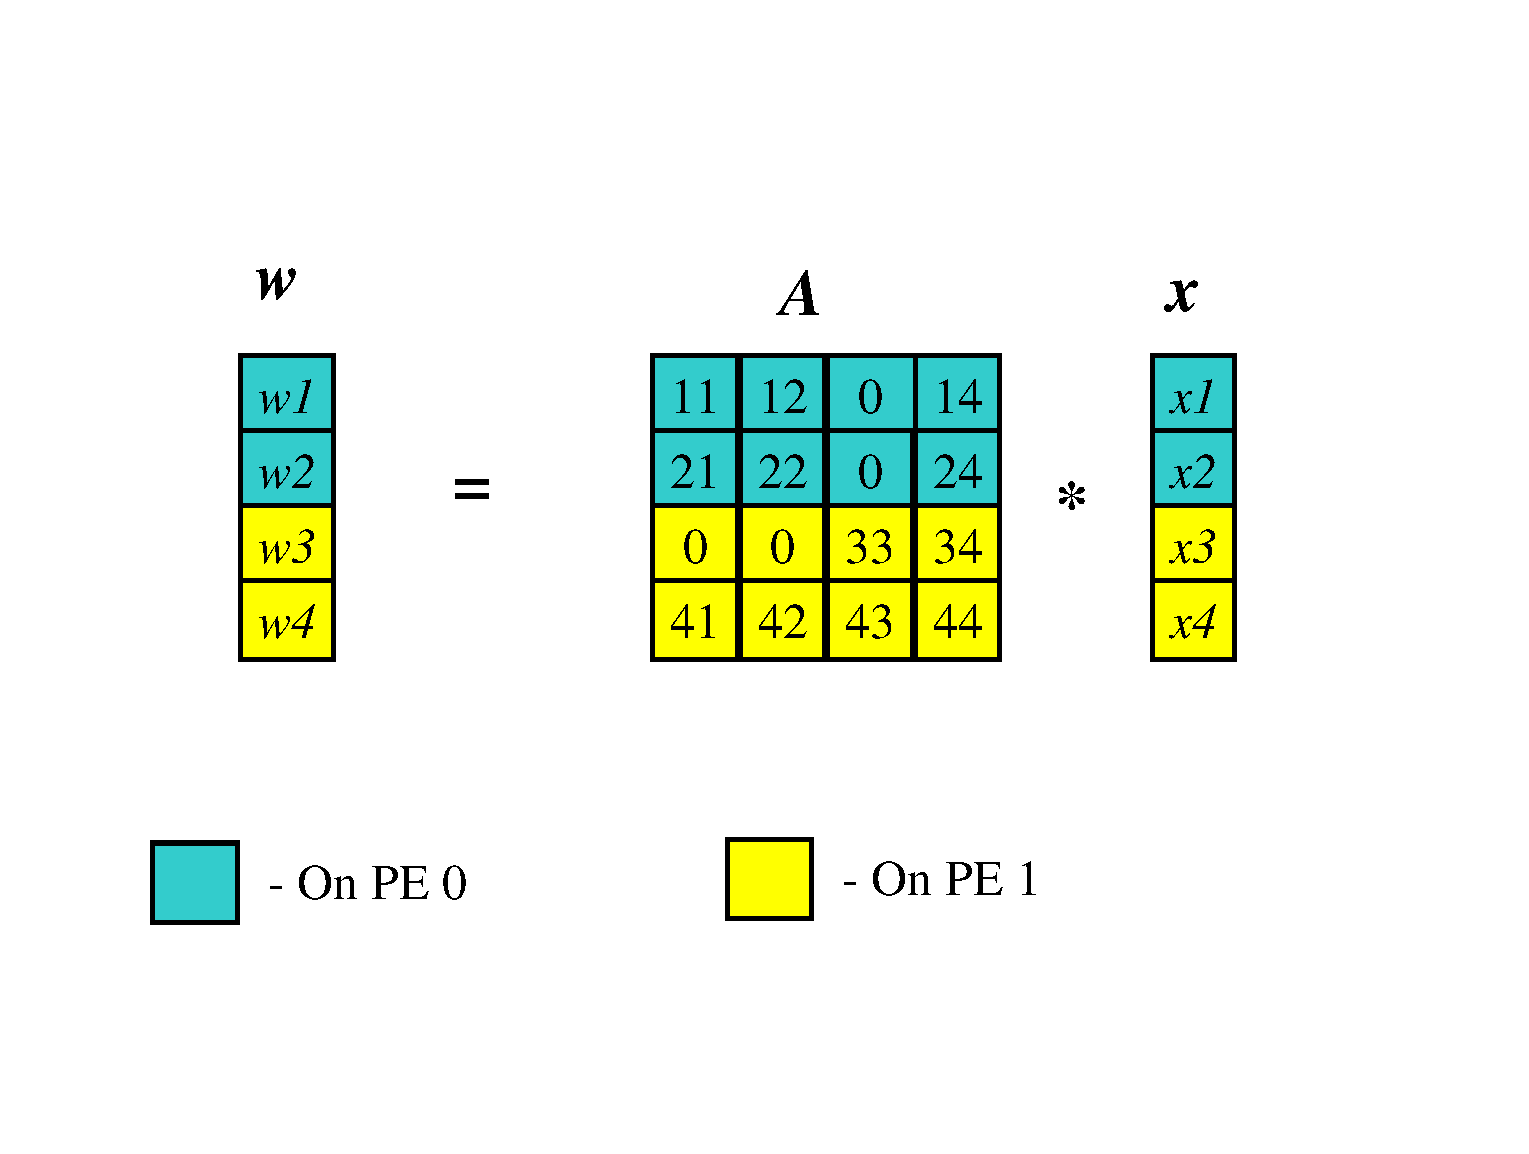
\includegraphics[height=3in]{TwoPESpMV}
\end{center} 
\label{MatrixVectorDistribution}
\caption{Matrix and vector assigments on two memory images}
\end{figure} 

\begin{figure} 
\begin{center} 
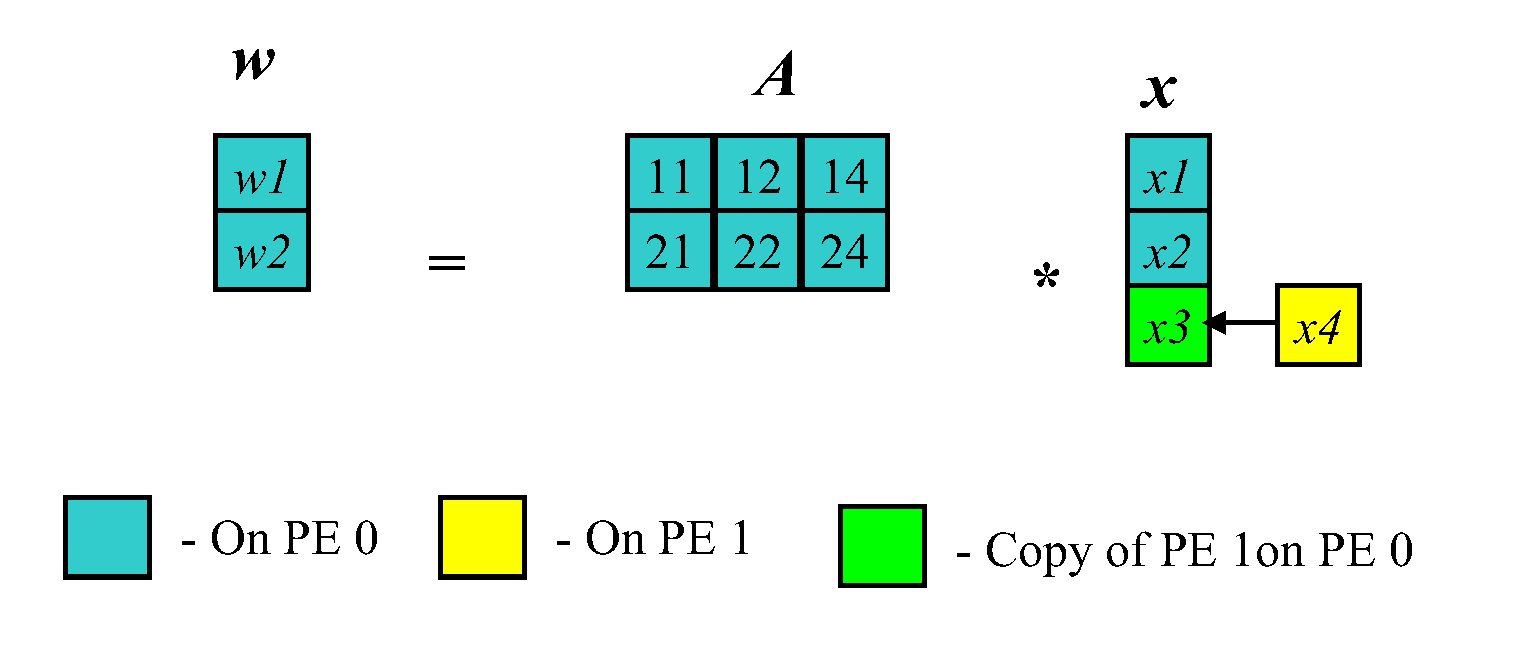
\includegraphics[height=3in]{PE0SpMV}
\end{center} 
\label{PE0MatrixVectorDistribution}
\caption{Contents of memory image on PE 0 after distribution}
\end{figure} 

\begin{figure} 
\begin{center} 
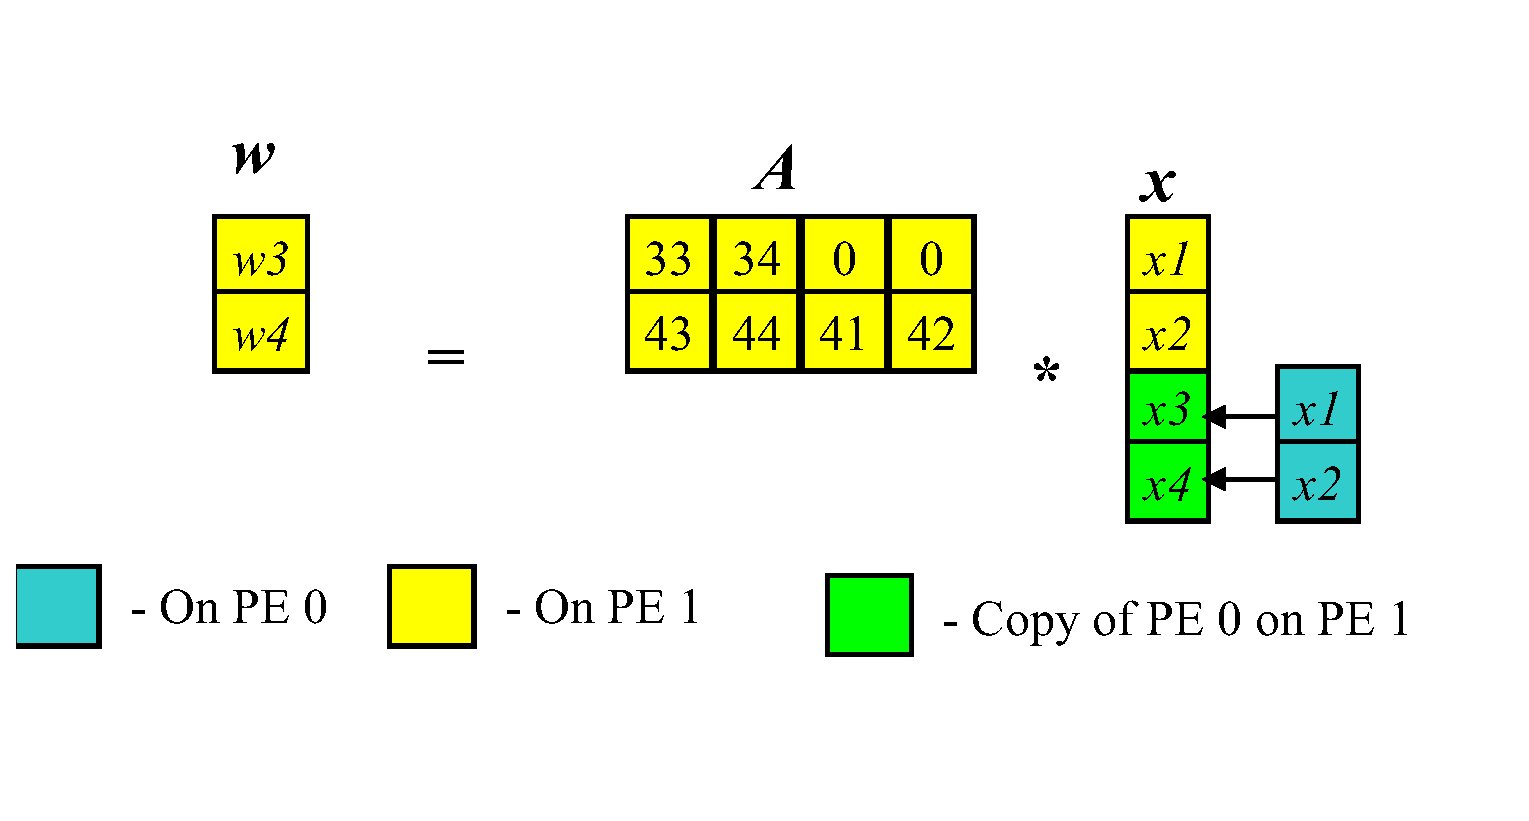
\includegraphics[height=3in]{PE1SpMV}
\end{center} 
\label{PE1MatrixVectorDistribution}
\caption{Contents of memory image on PE 1 after distribution}
\end{figure} 


\section{PDR Terms and Concepts}
\label{sect:concepts}

\subsection{Distributed Objects}

\subsection{Element Spaces and Global IDs}

Given an existing distribution of data, we want a formal mechanism for describing
how the data should be redistributed.  To accomplish this, we define an 
{\it element space} as a collection of labeled elements.  The exact meaning of
an element is determined by the type of object we are redistributing.
The label associated with each element is a signed integer value which we refer to as
the {\it global identifier} or {\it GID} of that element.  If there are no 
repeated GIDs associated with an element space, the element space is said to 
have the one-to-one property.  For many of the redistribution operations, the
one-to-one property is required for one or both of the element spaces involved
in the redistribution operation.

An element space is itself a distributed object.  An Espace is constructed by 
having each processor call the espace constructor, passing in the number of
elements that should be assigned to the processor and a list of related GIDs.

\subsection{Import and Export Operations}

\section{Important PDR Classes}

\subsection{Parallel Machine Class}

\subsection{Element Space Class}

\subsection{Distributed Object Base Class}

\subsection{User Oriented Distributed Object Classes}

\subsection{Import and Export Classes}

\subsubsection{Classification of Global IDs}


\section{Using Imports and Exports for Common PDR Operations}

\subsection{Sparse Matrix Vector Multiplication}

\subsection{Optimal Data Distributions}

\section{Conclusions}


% ---------------------------------------------------------------------- %
% References
%
\clearpage
\bibliographystyle{plain}
\bibliography{../CommonFiles/TrilinosBibliography}
\addcontentsline{toc}{section}{References}


\end{document}
